\section{Osservazione dei risultati }\label{se:prima-sezione}

Qui parlero con chiarezza di quanto sono i risutati aggingendo le varie immagini necessarie e del casa e del caso 
naturlamente mi asepetto di trovare qualche difficolta nell inserimento dei risultati  qui ma la bellezza di questo tipo di ragionamento 

\begin{figure}[tbp] 
\begin{center}
\begin{tabular}{c @{\hspace{1em}} c}
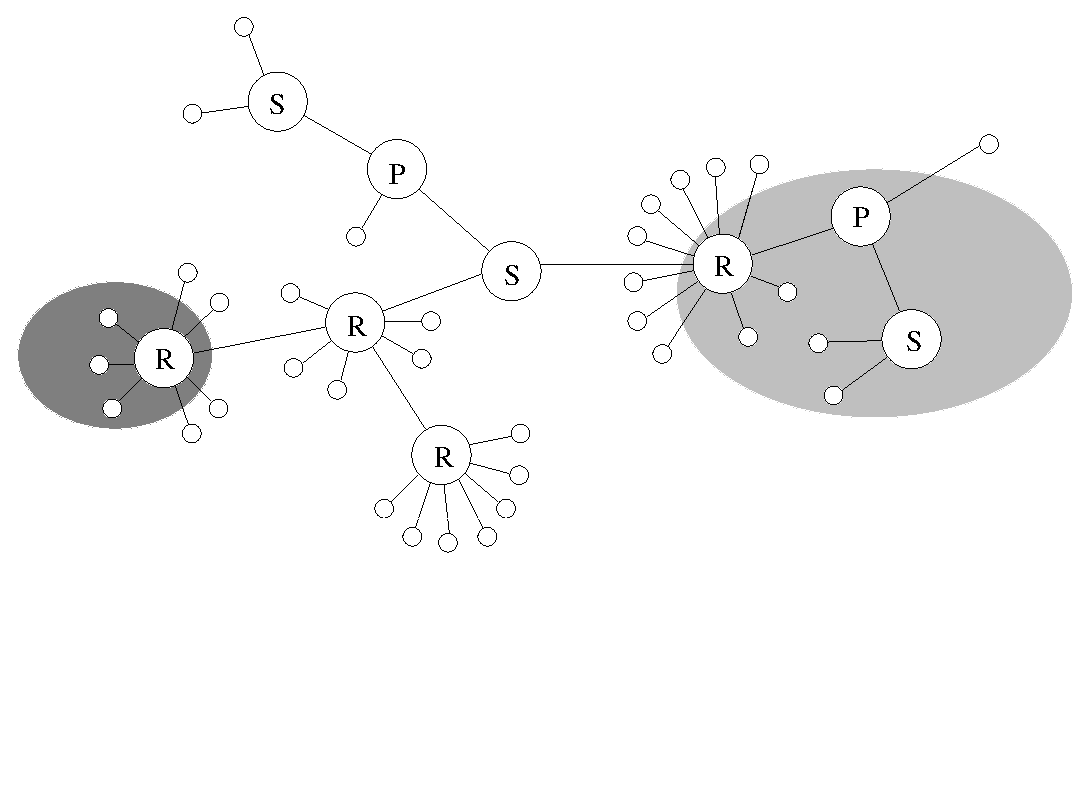
\includegraphics[width=8cm]{figure/esempio-figura-1.eps} &
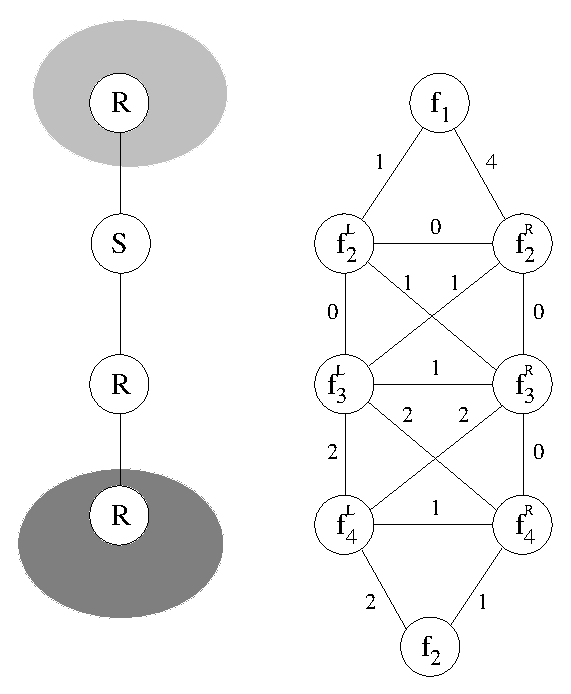
\includegraphics[width=5.5cm]{figure/esempio-figura-2.eps} \\
 (a) & (b)
\end{tabular}
\end{center}
\caption{SPQR-tree di un grafo. (a) L'albero di allocazione della faccia esterna. (b) Il cammino notevole di cui si parla tanto nella Sezione~\ref{se:prima-sezione}.} \label{fig:figura-doppia}
\end{figure}

Come si evince dalle Figure~\ref{fig:figura-doppia}.a e~\ref{fig:figura-doppia}.b non si capisce molto.
